\chapter{Appendix A}
\section{Balanced Detection: RIN Cancellation}
\label{appendix:RIN}
As discussed  in \autoref{sec:lit-noiseSources}, the best-case performance of a DWL system is for it to operate in a shot-noise limited regime - thus, all other sources of noise should be reduced to below the shot-noise level. In coherent detection LiDAR architectures, the use of a balanced detector setup has become common for this purpose, as it assists in reducing a laser source's relative-intensity noise (RIN) below the shot-noise level, in a manner which single-ended detection does not. 

A single-ended detection system simply uses a 2:1 (2 inputs, one output) fiber optic coupler to mix the LO reference signal with the backscatter signal, and uses a single photodetector to convert this light signal into a measurable current. It can be seen that this detection method retains the DC terms $P_{LO}$, $P_{RS}$. Any RIN from the laser source is present in the output, as these intensity fluctuations are contained in these two power terms. Thus, the measurable Doppler peak will be smaller with respect to the noise floor. 

Contrastingly, balanced detection setup makes use of a 2:2 fibre optic coupler which also optically mixes the LO reference signal with the received backscatter signal (as discussed in \autoref{sec:lit-coherentDetection}). However, the 2:2 coupler has two outputs, thus giving two output signals which can be termed $E_1$ and $E_2$ \cite{kikuchi_fundamentals_2016}:

\begin{equation}
	E_1 = \frac{1}{\sqrt2}(E_{RS} + E_{LO}), \space 
	E_2 = \frac{1}{\sqrt{2}}(E_{RS} - E_{LO})
\end{equation}
Where $E_{RS}$ and $E_{LO}$ are the complex electromagnetic fields of the returned backscatter signal and the local oscillator respectively. 

Thereafter, the two signals enter the balanced detector, which consists of two matched photodiodes and a transimpedance amplifier to convert their currents into a measurable voltage. The photodiodes respond with currents $I_1$ and $I_2$ respectively, proportional to the intensity of the electromagnetic field incident on it ($|E_{1}|^2$ and $|E_2|^2$ respectively), as was also discussed in \autoref{sec:lit-coherentDetection}. Due to the internal setup of the transimpedance amplifier and the photodiodes in the balanced detector, the output current is then given by \cite{kikuchi_fundamentals_2016}:

\begin{equation}
	I_{det} \propto I_1 - I_2 \propto |E_1|^2 - |E_2|^2 \newline
	\propto 2\sqrt{P_{LO}P_{RS}} cos(2\pi\Delta f t)
\end{equation}

Comparing this to \autoref{eqn:beatSignal}, it can be seen that the DC terms $P_{LO}$ and $P_{RS}$ are no longer present due to them being common-mode in both $I_1$ and $I_2$ and thus being canceled by the subtraction. This therefore lowers the noise floor, as the RIN contained in these terms is also eliminated. 

\autoref{fig:balanceddetector} depicts this process graphically:
\begin{figure}[H]
	\centering
	\begin{tikzpicture}[font=\small, line width=0.7pt]
		
		% ---- inputs ----
		\draw[->] (0.3,2.25) -- (2.2,2.25);
		\node[above] at (1.25,2.25) {$E_{LO}$ (LO)};
		\draw[->] (0.3,0.75) -- (2.2,0.75);
		\node[below, align=center] at (1.25,0.75) {$E_{RS}$\\(backscatter)};
		
		% ---- coupler ----
		\draw[rounded corners=2pt] (2.2,0.25) rectangle (4.0,2.75);
		\node[align=center] at (3.1,1.5) {50:50\\coupler};
		
		% ---- coupler outputs ----
		\draw[->] (4.0,2.25) -- (9.0,2.25);
		\node[above] at (6.5,2.25) {$E_1 = \tfrac{1}{\sqrt{2}}(E_{RS} + E_{LO})$};
		\draw[->] (4.0,0.75) -- (9.0,0.75);
		\node[below] at (6.5,0.75) {$E_2 = \tfrac{1}{\sqrt{2}}(E_{RS} - E_{LO})$};
		
		% ---- balanced detector ----
		\draw[rounded corners=2pt] (9.0,-0.25) rectangle (12.0,3.25);
		\node[above] at (10.5,3.25) {Balanced detector};
		\draw[rounded corners=1pt] (9.3,1.85) rectangle (10.5,2.65);
		\node at (9.9,2.25) {PD$_1$};
		\draw[rounded corners=1pt] (9.3,0.35) rectangle (10.5,1.15);
		\node at (9.9,0.75) {PD$_2$};
		
		% ---- difference ----
		\draw (10.5,2.25) -- (11.0,2.25) -- (11.0,0.75) -- (10.5,0.75);
		\node[above, font=\footnotesize] at (10.75,2.25) {$I_1$};
		\node[below, font=\footnotesize] at (10.75,0.75) {$I_2$};
		\fill (11.0,1.5) circle (1.5pt);
		\draw (11.0,1.5) -- (12.0,1.5);
		
		% ---- output ----
		\draw[->] (12.0,1.5) -- (12.7,1.5);
		\node[right] at (12.7,1.5) {$I_1 - I_2$};
	\end{tikzpicture}
	\caption{Balanced detection. The 50:50 coupler delivers the sum and difference
		of the backscatter and LO fields to two matched photodiodes; the output is the
		difference of their photocurrents, in which the common-mode terms cancel and
		only the beat term $2\sqrt{P_{LO} P_{RS}}\cos(2\pi\Delta f t)$ remains.}
	\label{fig:balanceddetector}
\end{figure}

It can thus be seen that balanced detection provides the advantage of cancelling RIN. This allows for the final detected signal to theoretically be able to achieve the desired shot-noise limited operation (if other sources of noise are also eliminated). 

\section{A3: Supplementary Experiment on RIN Cancellation}
\label{appendix:RINValidation}
\autoref{fig:A3Plot} gives the 5 - 20MHz averaged PSD of the detected noise, when only a single photodetector input of the PD100B is used - effectively turning it into a singe-ended detector. The electronic noise floor will remain the same, but the total noise PSD averages will now also contain RIN in addition to shot-noise and electronic noise. Before analysis of this plot can commence, it is important to note that in the case of balanced detection, the shot-noise of each detector is uncorrelated, and will therefore add together at the output. Thus, in the single-ended case, the shot-noise at the output for a given laser current is expected to be half that of the balanced detection case. Any excess noise above this half-power shot-noise level is thus contributed from the electronic noise, and the uncancelled RIN. 

\begin{figure}[H]
	\centering
	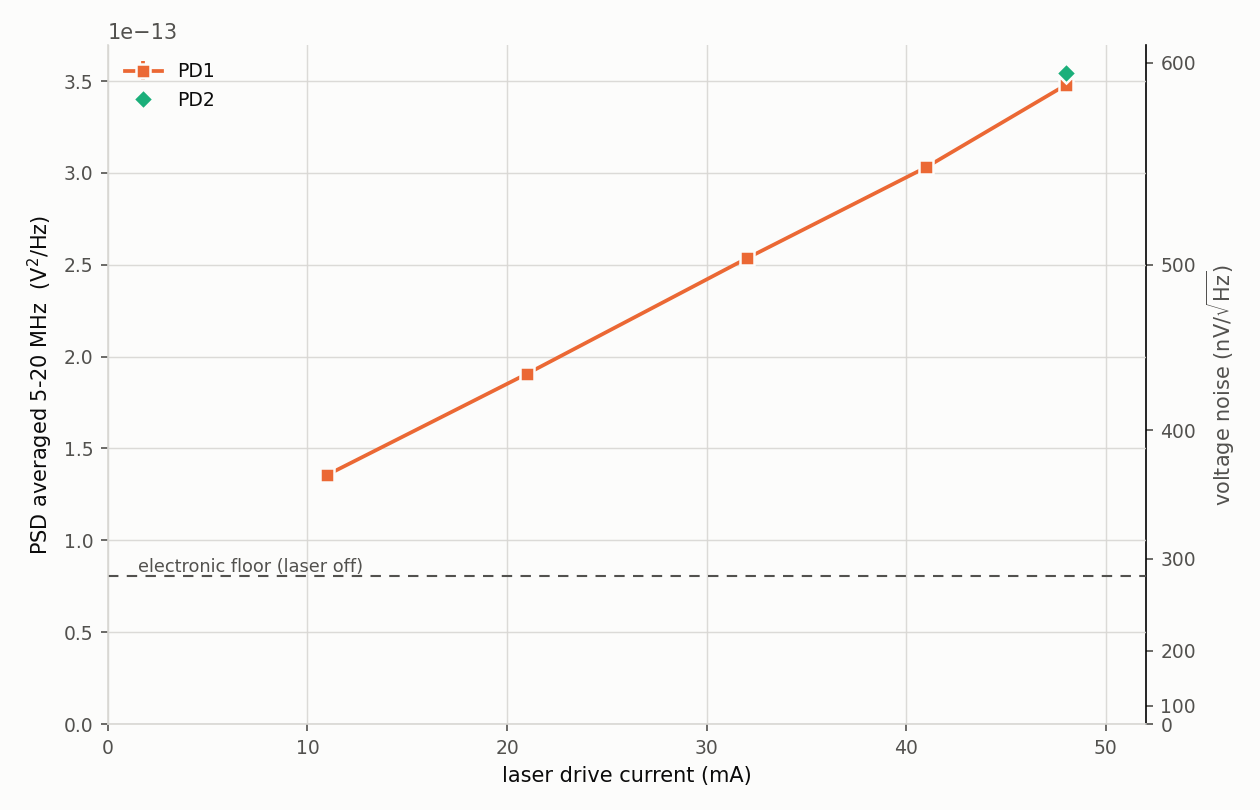
\includegraphics[width=1\linewidth]{psd_vs_current_single.png}
	\caption{A3: 5 - 20MHz Average PSD vs Laser Current with Single-Ended Detection}
	\label{fig:A3Plot}
\end{figure}

It can be seen in \autoref{fig:A3Plot} that indeed, the total noise is lower than in \autoref{fig:A2PSDvsCurrent}, as expected. Observing the total noise at the operating point of 48mA however, it can be seen that a value of approximately $3.5 \times 10^{-13}V^2/Hz$ is obtained, which gives $2.694\times 10^{-13}V^2/Hz$ once electronic noise has been subtracted. In the balanced detection case at the same laser current, a value of $5.49\times10^{-13}V^2/Hz$ was obtained - subtracting electronic noise and halving this gives $2.342\times 10^{-13}V^2/Hz$. This clearly indicates that the noise power in the single-ended case is higher than simply half of the shot-noise in the balanced detection case, thus proving that indeed there is excess RIN present. This excess RIN noise can be calculated: 
\begin{equation}
	RIN_{excess}= (2.694 - 2.342)\times 10^{-13} = 0.352\times 10 ^{-13}V^2/Hz
\end{equation}

Converting to dB:

\begin{equation}
	10log_{10}(1+\frac{RIN_{excess}}{S})=10log_{10}(1+\frac{0.352\times 10 ^{-13}}{2.324\times 10^{-13}})= 0.6125dB
\end{equation}

Thus, RIN contributes an additional 0.6125dB of noise above the ideal shot-noise limit at the 48mA operating point. Balanced detection allows this excess noise to be removed, as illustrated in the results of A2 - allowing for a better SNR.

\section{Linewidth, PIIN and Doppler peak broadening}
\label{appendix:PIIN}
In order to understand the linewidth property of a laser source, it is important to first have an understanding of the concept of phase noise in a laser:

    An ideal laser emits an electromagnetic wave $E(t) = E_0cos(2\pi f_0t + \phi)$ with $\phi$ a constant. A real laser emits $E(t)=E_0cos(2\pi f_0t + \phi(t))$ where $\phi(t)$ drifts unpredictably. This drift is called phase noise. Thus, when considering the frequency spectrum of the emitted laser beam over a long time period, it takes a Lorentzian shape centred around the nominal frequency of the laser (whereas an ideal laser would present simply as a delta spike at the nominal frequency). The laser linewidth, $\Delta f$, is then defined as the -3dB bandwidth of this Lorentzian spectrum, as illustrated in \autoref{fig:lorentzian} below:

    \begin{figure}[H]
    \centering
    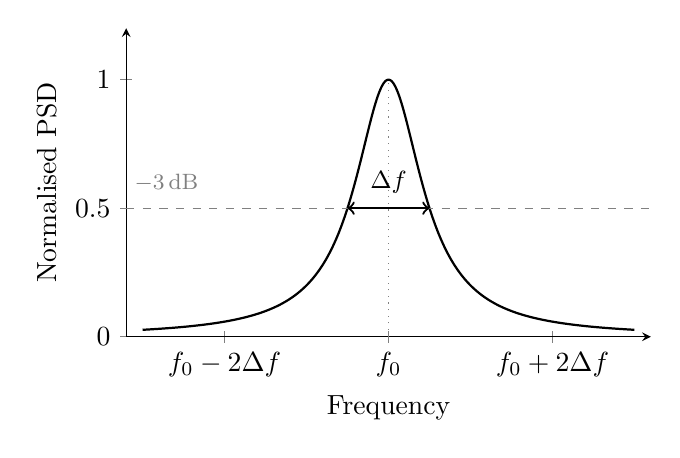
\begin{tikzpicture}
    \begin{axis}[
        width=0.68\textwidth, height=5.5cm,
        xlabel={Frequency},
        ylabel={Normalised PSD},
        domain=-3:3, samples=400,
        xmin=-3.2, xmax=3.2, ymin=0, ymax=1.2,
        axis lines=left,
        xtick={-2,0,2},
        xticklabels={$f_0-2\Delta f$, $f_0$, $f_0+2\Delta f$},
        clip=false,
    ]
    \addplot[thick, black] {1/(1+(2*x)^2)};
    
    % half-maximum level
    \addplot[dashed, gray] coordinates {(-3.2,0.5) (3.2,0.5)};
    \node[left, gray, font=\footnotesize] at (axis cs:-2.2,0.6) {$-3$\,dB};
    
    % centre line
    \draw[dotted, gray] (axis cs:0,0) -- (axis cs:0,1);
    
    % FWHM arrow
    \draw[<->, thick] (axis cs:-0.5,0.5) -- (axis cs:0.5,0.5);
    \node[above, font=\small] at (axis cs:0,0.52) {$\Delta f$};
    \end{axis}
    \end{tikzpicture}
    \caption{Lorentzian frequency spectrum of a laser diode.}
    \label{fig:lorentzian}
    \end{figure}

    Asssociated with the linewidth is a quantity termed coherence length. The coherence length of the emitted beam, $L_c$, is given by \cite{bennett_doppler_2003}:
    
    \begin{equation}
        L_c = \frac{c}{2\pi\Delta f}
        \label{eqn:coherenceLength}
    \end{equation}

    Where $\Delta f$ is the linewidth of the source laser, and $c$ is the speed of light. The coherence length is of relevance when considering linewidth effects. 
    
    The non-ideal linewidth property of a laser source gives rise to two primary effects in a DWL system's measurements - namely phase-induced intensity noise (PIIN), and the broadened Doppler peak:

    As noted by Cariou et al. \cite{cariou2006laser}, Jiang et al. \cite{jiang_performance_2019}, and Harris et al. \cite{harris_role_1998}, reflections of the outgoing beam - caused by optics and the fibre optic transmit path - travel back in the system and are interfered with the reference beam (LO) before detection (in the same way as the actual backscattered signal of interest is). Because the reflection and LO derive
    from the same source, the mixing product is a strong, unwanted tone at baseband (homodyne)
    or at the intermediate frequency (heterodyne), carrying the phase noise
    accumulated over the path-length mismatch $\Delta L$ between the reflection and the LO. Harris et
    al. \cite{harris_role_1998} show that the form of this residual noise is set by how large
    $\Delta L$ is relative to the coherence length ($L_c$) of the laser source. 
    
    For $\Delta L \gg L_c$ the two
    phases are highly uncorrelated because the difference in path (and therefore time) taken has allowed the phase of the two to "wander" significantly - and thus the tone broadens into a Lorentzian of width
    $2\Delta f$. This case is illustrated in \autoref{fig:commonmode} below, where it can be seen that this unwanted Lorentzian peak can serve to swamp out the desired Doppler peak to be measured - this is especially impactful for low wind-speeds, where the Doppler peak will be closer to the unwanted common-mode Lorentzian peak, and will be hidden more by it.

    \begin{figure}[H]
    \centering
    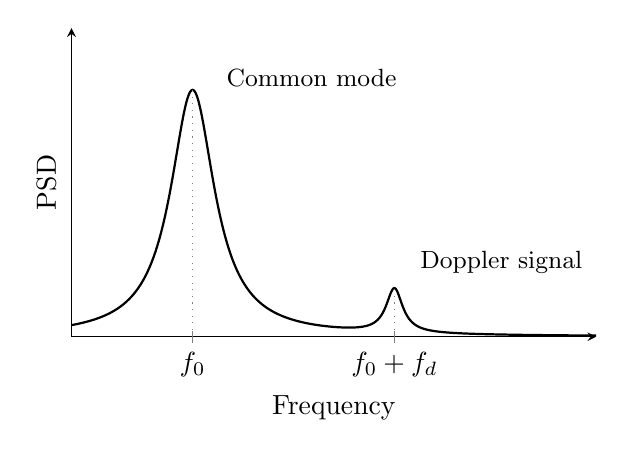
\begin{tikzpicture}
    \begin{axis}[
        width=0.68\textwidth, height=5.5cm,
        xlabel={Frequency},
        ylabel={PSD},
        domain=-1.5:5, samples=500,
        xmin=-1.5, xmax=5, ymin=0, ymax=1.25,
        axis lines=left,
        xtick={0,2.5},
        xticklabels={$f_0$, $f_0+f_d$},
        ytick=\empty,
        clip=false,
    ]
    % common mode + Doppler signal
    \addplot[thick, black] {1/(1+(3*x)^2) + 0.18/(1+(8*(x-2.5))^2)};

    % centre lines
    \draw[dotted, gray] (axis cs:0,0) -- (axis cs:0,1);
    \draw[dotted, gray] (axis cs:2.5,0) -- (axis cs:2.5,0.2);

    % peak labels
    \node[right, font=\small] at (axis cs:0.3,1.05) {Common mode};
    \node[right, font=\small] at (axis cs:2.7,0.3) {Doppler signal};
    \end{axis}
    \end{tikzpicture}
    \caption{Spectrum of a monostatic CW coherent lidar, showing the Doppler
    signal superimposed on the skirt of the common-mode peak (adapted from \cite{cariou2006laser}).}
    \label{fig:commonmode}
    \end{figure}
    
    For $\Delta L \ll L_c$, the case where the mismatch between LO and reflection paths is smaller, the reflected signal and the LO will be more correlated in phase.
    Thus, the residual instead appears as a flat excess noise floor across the
    frequency band, of level proportional to $\Delta f\,\Delta L^{2}$
    \cite{harris_role_1998}. This excess noise is termed excess LO noise,
    interferometric noise or phase-induced intensity noise (PIIN), depending on author
    \cite{harris_role_1998,abari_all-fiber_2014,jiang_performance_2019}. For the remainder of this paper, this excess noise will be termed PIIN. PIIN has
    been measured at 5 - 30dB above shot noise in a diode-laser
    lidar \cite{harris_role_1998} and well above shot noise in a fibre-laser
    system \cite{jiang_performance_2019}. Thus, PIIN is a significant noise source which can cause the system to operate far from the ideal shot-noise limit discussed in \autoref{sec:lit-noiseSources}. It is thus clear that to reduce PIIN, a laser with as small a linewidth as possible should be selected, and the path length mismatch, $\Delta L\ L$ between LO and reflection paths should be minimised. 

    Another consideration arising due to non-ideal laser linewidth is the broadening of the measurable Doppler peak. This is particularly notable for longer ranges. 
    
    If the coherence length from \autoref{eqn:coherenceLength} is long relative to the emitted signal's path length, the broadening of the Doppler peak due to the laser's linewidth may be neglected, and it will instead be other factors (such as turbulence in the air, and speckle) which dominate and cause a broader measurable peak \cite{bennett_doppler_2003}. This is because the total round-trip time of the beam is shorter, thus ensuring that the phase of the beam has not had "time" to shift significantly in between transmission, and later reception and mixing with the local oscillator. Thus, the received backscatter signal and the LO phase will be more coherent and will result in a sharper peak after mixing.
    
    Conversely, if the coherence length is short relative to the signal path length (i.e. for targets at greater ranges), the Doppler peak will be spread over $2\times\Delta f$, meaning that the measurement resolution and the ability to resolve turbulence in the air will be reduced \cite{bennett_doppler_2003}.

    From the two effects described above, it can clearly be seen that a narrow linewidth laser source is highly beneficial for DWL systems, in order to achieve the best-case shot-noise limited operation, and to achieve a narrow, measurable Doppler peak. 


\textbf{IMPORTANT:} Appendix A (see the table below) should provide a summary of how you have met the GAs associated with the course, and where in the report the evidence can be found.

If you have used AI in writing your report, you need to provide details in one of the appendices of how you used it.

If appropriate, in a subsequent appendix, provide a link to any GitHub repository where the code and additional materials for your project can be found.

\section{D: Wind-tunnel tests full results}
\label{appendix:FullWTResults}
\begin{figure}
	\centering
	\includegraphics[width=1\linewidth]{"../Data Acquisition/figures/psd_windtunnel_cases"}
	\caption{Grid of PSD plots for each wind-tunnel setpoint}
	\label{fig:psdwindtunnelcases}
\end{figure}


\begin{center}
\begin{tabular}{||p{2em} |p{15em} |p{20em}||}
 \hline
 \textbf{GA} & \textbf{Requirement} & \textbf{Justification and section in the report}  \\ [0.5ex] 
 \hline\hline
 1 & Problem-solving & Description here  \\ 
 \hline
 4 & Investigations, experiments and data analysis & Description here  \\
 \hline
 5 & Use of engineering tools & Description here \\
 \hline
 6 & Professional and technical communication (Long report) & Description here \\
 \hline
 8 & Individual work & Description here \\
 \hline
 9 & Independent learning ability & Description here \\ [1ex] 
 \hline
\end{tabular}
\end{center}
